\documentclass[../practica.root.tex]{subfiles}

\newcommand{\gravity}[1][per-mode=fraction]{\SI[#1]{9,8}{\meter\per\second\squared}}

\begin{document}

\section{Unidad 7}
\subsection{Parte 1}
\begin{enumerate}
	\item
	      \begin{multicols}{2}
		      Guillermo entrena arrastrando \SI{20}{\meter} una bigornia que
		      está vinculada a su cintura por medio de una soga como
		      muestra la figura. El ángulo que forma la soga con el piso es
		      de \ang{35} y la fuerza que ejerce Guillermo es de \SI{420}{\newton}. Si una
		      fuerza de fricción de \SI{320}{\newton} se opone al movimiento.
		      Calcule el trabajo total realizado.
		      \begin{center}
			      \begin{tikzpicture}[scale=1.1]
				      \draw (-0.5,-0.5) rectangle ++(1,1);
				      \filldraw[red] (0,0) circle [radius=0.05];
				      \begin{scope}[fvec, near end] % Vectores
					      \draw (0,0) -- node[above]{$\vec{F}_a$} (35:2) node(F){};
					      \draw (0,0) -- node[above]{$\vec{f}_k$} (-1.5,0);
				      \end{scope}
				      % Angulo
				      \draw[help lines] (0,0) -- (F |- 2,0);
				      \draw[help lines] (0.7,0) arc[start angle=0, end angle=35, radius=0.7] node[pos=0.5, right]{$\theta$};
				      % Desplazamiento
				      \draw[gray!70, very thin] (-3,0) ++(-0.5,-0.5) rectangle ++(1,1);
				      \draw[dashed, |->] (-3,-1) -- node[below]{$\vec{s}$}(0,-1);
			      \end{tikzpicture}
		      \end{center}
	      \end{multicols}
	      \begin{center}
		      \[ W = \vec{s}\cdot\vec{F} \]
		      \[ F_x = F_a\cos\theta - f_s \]
		      \[ F_x = \SI{344}{\newton} - \SI{320}{\newton} \]
		      \[ F_x = \SI{24}{\newton} \]
		      \[ W_x = \SI{20}{\meter}\cdot\SI{24}{\newton} \]
		      \[ \boxed{W_x = \SI{480}{\joule}} \]
	      \end{center}

	\item
	      \begin{multicols}{2}
		      Dos bloques están unidos por una cuerda muy ligera que pasa por una polea sin masa y
		      sin fricción, como muestra la figura. Los bloques se están desplazando a rapidez
		      constante, el bloque A de \SI{20}{\newton} se mueve \SI{75,0}{\centi\meter} hacia la derecha y
		      el bloque B de \SI{12,0}{\newton} se mueve \SI{75,0}{\centi\meter} hacia abajo. Durante el proceso, \\ \\
		      \begin{center}
			      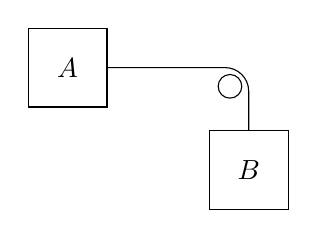
\begin{tikzpicture}
				      \draw (-0.5,0.5) rectangle ++(1,1) node[midway](A){$A$};
				      \draw (A) ++(0.5,0) -- ++(1.5,0) arc(90:0:0.3) node[midway](c){} -- ++(0,-0.5) node(B){};
				      \draw (B) ++(0.5,0) rectangle ++(-1,-1) node[midway]{$B$};
				      \draw (c) ++(-0.15,-0.15) circle[radius=0.15];
			      \end{tikzpicture}
		      \end{center}
	      \end{multicols}
	      \begin{enumerate}
		      \item ¿Cuánto trabajo efectúan sobre el bloque B: la gravedad y la tensión de la cuerda?
		            \begin{center}
			            \[ W_g = s_y\cdot F_g \]
			            \[ W_g = \SI{0,75}{\meter}\cdot\SI{12,0}{\newton} \]
			            \[ \boxed{W_g = \SI{9,0}{\joule}} \]

			            \[ \sum F_y = \SI{0}{\newton} \]
			            \[ \sum F_y = F_g + T_c = \SI{0}{\newton} \]
			            \[ \SI{12,0}{\newton} + T_c = \SI{0}{\newton} \]
			            \[ T_c = \SI{-12,0}{\newton} \]
			            \[ W_c = s_y\cdot T_C \]
			            \[ W_c = \SI{0,75}{\meter}\cdot\SI{-12,0}{\newton} \]
			            \[ \boxed{W_c = \SI{-9,0}{\joule}} \]

		            \end{center}
		      \item ¿Cuánto trabajo efectúan sobre el bloque A: la gravedad, la tensión de la cuerda, la fricción y la fuerza normal?
		            \begin{center}
			            \[ W_g = s_y\cdot F_g \]
			            \[ W_g = \SI{0}{\meter}\cdot\SI{20}{\newton} \]
			            \[ \boxed{W_g = \SI{0}{\joule}} \]

			            \[ W_c = s_x\cdot T_c \]
			            \[ W_c = \SI{0,75}{\meter}\cdot\SI{12,0}{\newton} \]
			            \[ \boxed{W_c = \SI{9,0}{\joule}} \]

			            \[ a_x = 0 \Rightarrow F_x = \SI{0}{\newton} \]
			            \[ \sum F_x = \SI{0}{\newton} \]
			            \[ \sum F_x = T_c + f_k = \SI{0}{\newton} \]
			            \[ \SI{12,0}{\newton} + f_k = \SI{0}{\newton} \]
			            \[ f_k = \SI{-12,0}{\newton} \]
			            \[ W_f = s_x\cdot\SI{-12,0}{\newton} \]
			            \[ W_f = \SI{0,75}{\meter}\cdot\SI{-12,0}{\newton} \]
			            \[ \boxed{W_f = \SI{-9,0}{\joule}} \]

			            \[ W_n = s_y\cdot F_n \]
			            \[ W_n = \SI{0,0}{\meter}\cdot\SI{20}{\newton} \]
			            \[ \boxed{W_n = \SI{0}{\joule}} \]
		            \end{center}
		      \item Obtenga el trabajo total efectuado sobre cada bloque. \\
		            Para el bloque B:
		            \begin{center}
			            \[ \sum F_x = \SI{0}{\newton} \]
			            \[ \sum F_y = F_g - T_c \]
			            \[ \sum F_y = \SI{12,0}{\newton} - \SI{12,0}{\newton} \]
			            \[ \sum F_y = \SI{0,0}{\newton} \]
			            \[ W = \vec{s}\cdot\vec{F} \]
			            \[ W = \SI{0,75}{\meter}\vec{i}\cdot\SI{0,0}{\newton}\vec{i} \]
			            \[ \boxed{W = \SI{0,0}{\joule}} \]
		            \end{center}
		            Para el bloque A:
		            \begin{center}
			            \[ \sum F_x = T_c + f_k \]
			            \[ \sum F_x = \SI{12,0}{\newton} + \SI{-12,0}{\newton} \]
			            \[ \sum F_x = \SI{0,0}{\newton} \]
			            \[ \sum F_y = F_g + F_n \]
			            \[ \sum F_y = \SI{20}{\newton} + \SI{-20}{\newton} \]
			            \[ \sum F_y = \SI{0}{\newton} \]
			            \[ W = \vec{s}\cdot\vec{F} \]
			            \[
				            W = \SI{0,75}{\meter}\vec{i}\cdot\SI{0,0}{\newton}\vec{i}
				            + \SI{0}{\meter}\vec{j}\cdot\SI{0}{\newton}\vec{j}
			            \]
			            \[
				            W = \SI{0,0}{\joule}
				            + \SI{0}{\joule}
			            \]
			            \[ \boxed{W = \SI{0}{\joule}} \]
		            \end{center}
	      \end{enumerate}

	\item Considere una situación igual a la del problema anterior, pero suponga ahora que no hay
	      fuerza de rozamiento sobre el bloque A de \SI{20,0}{\newton} que descansa sobre la mesa. La polea
	      es ligera y sin fricción.
	      \begin{enumerate}
		      \item Calcule la tensión T en la cuerda ligera que une los bloques
		      \item Para un desplazamiento en el cual el bloque de \SI{12,0}{\newton} desciende \SI{1,20}{\meter},
		            calcule el trabajo total realizado sobre: el bloque A y el bloque B.
		      \item Para el desplazamiento del inciso b), calcule el trabajo total realizado sobre el sistema
		            de dos bloques. ¿Cómo se compara su respuesta con el trabajo realizado sobre el bloque
		            de \SI{12,0}{\newton} por la gravedad?
		      \item Si el sistema se libera del reposo, ¿cuál es la rapidez del bloque de \SI{12,0}{\newton} cuando ha
		            descendido \SI{1,20}{\meter}?

	      \end{enumerate}

	\item Un vagón de juguete con masa de \SI{7,00}{\kilo\gram} se mueve en línea recta sobre una superficie
	      horizontal sin fricción. Tiene una rapidez inicial de \SI[per-mode=fraction]{4,00}{\meter\per\second} y luego es empujado a lo
	      largo de \SI{3}{\meter}, en la dirección de la velocidad inicial, por una fuerza cuya magnitud es de
	      \SI{10,0}{\newton}.
	      \begin{enumerate}
		      \item Use el teorema de trabajo y energía para calcular la rapidez final del vagón
		            \begin{center}
			            \[ W = K_2 - K_1\ \text{(Teorema de trabajo-energía)} \]
			            \[ K = \frac{1}{2}mv^2\ \text{(Energía cinética)} \]
			            \[ W = Fs \]
			            \[ Fs = \frac{1}{2}m{v_2}^2 - \frac{1}{2}m{v_1}^2 \]
			            \[ v_1 = \SI{4}{\meter\per\second} \]
			            \[ s = \SI{3}{\meter} \]
			            \[ F = \SI{10,0}{\newton} \]
			            \[
				            \SI{10,0}{\newton}\cdot\SI{3}{\meter} =
				            \frac{1}{2}\cdot\SI{7,00}{\kilo\gram}(v_2)^2
				            - \frac{1}{2}\cdot\SI{7,00}{\kilo\gram}(\SI{4}{\meter\per\second})^2
			            \]
			            \[ \SI{30,0}{\newton\meter} = \SI{3,50}{\kilo\gram}((v_2)^2 - (\SI{4}{\meter\per\second})^2) \]
			            \[
				            \frac{ \SI{30,0}{\kilo\gram\meter\per\second\squared\meter} }
				            { \SI{3,50}{\kilo\gram} }
				            = (v_2)^2 - \SI{16}{\meter\squared\per\second\squared}
			            \]
			            \[
				            \SI{60/7}{\meter\squared\per\second\squared} = (v_2)^2 - \SI{16}{\meter\squared\per\second\squared}
			            \]
			            \[ \frac{60+16\cdot 7}{7}(\si{\meter\per\second})^2 = (v_2)^2 \]
			            \[ \frac{172}{7}(\si{\meter\per\second})^2 = (v_2)^2 \]
			            \[ \sqrt{\num{24,57}(\si{\meter\per\second})^2} = v_2 \]
			            \[ \boxed{v_2 = \SI{4,96}{\meter\per\second}} \]
		            \end{center}
		      \item Calcule la aceleración producida por la fuerza y úsela para calcular la rapidez final
		            del vagón con la fórmula utilizada en cinemática. Compare este resultado con el del
		            inciso a).
		            \begin{center}
			            \[ F = ma \]
			            \[ \SI{10,0}{\newton} = a \]
			            \[ \frac{\SI{10,0}{\kilo\gram\meter\per\second\squared}}{\SI{7,00}{\kilo\gram}} = a  \]
			            \[ a = \SI{1,42}{\meter\per\second\squared}\]
			            \[ \Delta X = V_it + \frac{1}{2}at^2 \]
			            \[ \SI{3}{\meter} = \SI{4,00}{\meter\per\second}t + \frac{1}{2}\SI{1,42}{\meter\per\second\squared}t^2 \]
			            \[ 0 = \SI{0,71}{\meter\per\second\squared}t^2 + \SI{4,00}{\meter\per\second}t + \SI{-3}{\meter} \]
			            \[
				            t_{1,2} = \frac{
					            \SI{-4,00}{\m/\s} \pm \sqrt{ (\SI{-4,00}{\m/\s})^2 - \num{4}\SI{0,71}{\m/\s^2}(\SI{-3}{\m}) }
				            }{
					            \num{2}\cdot\SI{0,71}{\meter\per\second\squared}
				            }
			            \]\[
				            t_{1,2} = \frac{
					            \SI{-4,00}{\m/\s} \pm \sqrt{ \SI{16,00}{\m^2/\s^2} + \SI{8,52}{\m^2/\s^2} }
				            }{
					            \SI{1,42}{\m/\s^2}
				            }
			            \]\[
				            t_{1,2} = \frac{
					            \SI{-4,00}{\m/\s} \pm \sqrt{ \SI{24,52}{\m^2/\s^2} }
				            }{
					            \SI{1,42}{\m/\s^2}
				            }
			            \]\[
				            t_{1,2} = \frac{
					            \SI{-4,00}{\m/\s} \pm \SI{4,95}{\m/\s}
				            }{
					            \SI{1,42}{\m/\s^2}
				            }
			            \]
			            \begin{multicols}{2}
				            \begin{center}
					            \[
						            t_1 = \frac{
							            \SI{-4,00}{\m/\s} + \SI{4,95}{\m/\s}
						            }{
							            \SI{1,42}{\m/\s^2}
						            }
					            \]\[
						            t_1 = \frac{
							            \SI{0,95}{\m/\s}
						            }{
							            \SI{1,42}{\m/\s^2}
						            }
					            \]
					            \[ t_1 = \SI{0,67}{\s} \]
				            \end{center}
				            \begin{center}
					            \[
						            t_2 = \frac{
							            \SI{-4,00}{\m/\s} - \SI{4,95}{\m/\s}
						            }{
							            \SI{1,42}{\m/\s^2}
						            }
					            \]\[
						            t_2 = \frac{
							            \SI{-8,95}{\m/\s}
						            }{
							            \SI{1,42}{\m/\s^2}
						            }
					            \]\[
						            \cancel{t_2 = \SI{-6,30}{\s}}
					            \]
				            \end{center}
			            \end{multicols}
			            \[ V_f = \SI{4,00}{\meter\per\second} + \SI{1,42}{\meter\per\second\squared}\SI{0,67}{\s} \]
			            \[ \boxed{V_f = \SI{4,96}{\meter\per\second}} \]
		            \end{center}
	      \end{enumerate}

	\item A un auto a radiocontrol de masa \SI{2,00}{\kilo\gram} que avanza por una pista recta, se le aplica una
	      fuerza $F$ en la dirección del movimiento. La componente $x$ de la $F$ varía con la coordenada
	      $x$ del automóvil, como se indica en la figura. Calcule el trabajo efectuado por la fuerza $F$
	      cuando el auto se mueve de
	      \begin{center}
		      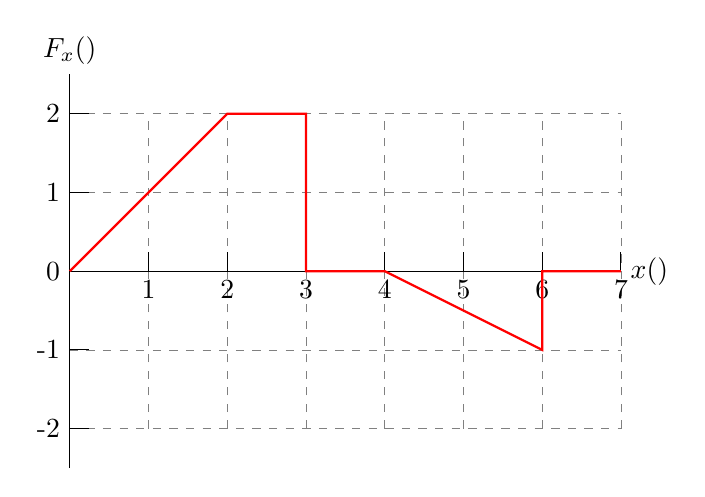
\begin{tikzpicture}
			      \draw[dashed, gray, very thin] (0,-2) grid (7,2);
			      % Referencia y ejes
			      \draw (0,-2.5) -- (0,2.5) node[above]{$F_x (\si{\newton})$}; % Eje Y
			      \foreach \y in {-2,...,2}
			      \draw (0, \y) node[left]{\y} -- +(0.25, 0);
			      \draw (0,0) -- (7,0) node[right]{$x (\si{\meter})$}; % Eje x
			      \foreach \x in {1,...,7}
			      \draw (\x, 0) node[below]{\x} -- +(0, 0.25);

			      \draw[red, thick] (0,0) -- (2,2) -- (3,2) -- (3,0) -- (4,0) -- (6,-1) -- (6,0) -- (7,0);
		      \end{tikzpicture}
	      \end{center}
	      \begin{multicols}{2}
		      \begin{enumerate}
			      \item $x = \SI{0}{\meter}$ a $x = \SI{3}{\meter}$
			            \[ W = \frac{\SI{2}{\meter}\cdot\SI{2}{\newton}}{2} + \SI{1}{\meter}\cdot\SI{2}{\newton} \]
			            \[ W = \frac{\SI{4}{\joule}}{2} + \SI{2}{\joule} \]
			            \[ \boxed{W = \SI{4}{\joule}} \]
			      \item $x = \SI{3}{\meter}$ a $x = \SI{4}{\meter}$
			            \[ W = \SI{1}{\meter}\cdot\SI{0}{\newton} \]
			            \[ \boxed{W = \SI{0}{\joule}} \]
			      \item $x = \SI{4}{\meter}$ a $x = \SI{7}{\meter}$
			            \[ W = \SI{2}{\meter}\cdot\SI{-1}{\newton} + \SI{1}{\meter}\cdot\SI{0}{\newton} \]
			            \[ \boxed{W = \SI{-2}{\joule}} \]
			      \item $x = \SI{0}{\meter}$ a $x = \SI{7}{\meter}$
			            \[ W_{0,2} = \frac{\SI{2}{\meter}\cdot\SI{2}{\newton}}{2} = \SI{2}{\joule} \] % (0 a 2)
			            \[ W_{2,3} = \SI{1}{\meter}\cdot\SI{2}{\newton} = \SI{2}{\joule} \] % (2 a 3)
			            \[ W_{3,4} = \SI{1}{\meter}\cdot\SI{0}{\newton} = \SI{0}{\joule} \] % (3 a 4)
			            \[ W_{4,6} = \frac{\SI{2}{\meter}\cdot\SI{-1}{\newton}}{2} = \SI{-1}{\joule} \] % (4 a 6)
			            \[ W_{6,7} = \SI{1}{\meter}\cdot\SI{0}{\newton} = \SI{0}{\joule} \] % (6 a 7)
			            \[ W_{0,7} = W_{0,2} + W_{2,3} + W_{3,4} + W_{4,6} + W_{6,7} \]
			            \[ W_{0,7} = (2 + 2 + 0 + \num{-1} + 0)\si{\joule} \]
			            \[ \boxed{W_{0,7} = \SI{3}{\joule}} \]
			      \item $x = \SI{7}{\meter}$ a $x = \SI{2}{\meter}$
			            \[ W_{7,6} = \SI{-1}{\meter}\cdot\SI{0}{\newton} = \SI{0}{\joule} \]
			            \[ W_{6,4} = \frac{\SI{-2}{\meter}\cdot\SI{-1}{\newton}}{2} = \SI{1}{\joule} \]
			            \[ W_{4,3} = \SI{-1}{\meter}\cdot\SI{0}{\newton} = \SI{0}{\joule} \]
			            \[ W_{3,2} = \SI{-1}{\meter}\cdot\SI{2}{\newton} = \SI{-2}{\joule} \]
			            \[ W_{7,2} =  W_{7,6} + W_{6,4} + W_{4,3} + W_{3,2} \]
			            \[ W_{7,2} = (0 + 1 + 0 + \num{-2})\si{\joule} \]
			            \[ \boxed{W_{7,2} = \SI{-1}{\joule}} \]

		      \end{enumerate}
	      \end{multicols}

	\item ¿Cuántos Joules de energía consume una lamparita eléctrica de \SI{100}{\watt} si permanece
	      prendida durante 1 hora? ¿Con qué rapidez tendría que correr una persona de \SI{70,0}{\kilo\gram} para
	      tener esa cantidad de energía como energía cinética?
	      \begin{center}
		      \[ \si{\joule} = \si{\watt\second} \]
		      \[ j = \SI{100}{\watt}\cdot\SI{3600}{\second} \]
		      \[ j = \SI{360000}{\joule} \]
		      \[ \boxed{j = \SI{360}{\kilo\joule}} \]

		      \[ K = \frac{1}{2}mv^2 \]
		      \[ \SI{360000}{\joule} = \frac{1}{2}\SI{70,0}{\kilo\gram}\cdot v^2 \]
		      \[ \SI{360000}{\kilo\gram(\meter\per\second)^2} = \SI{35,0}{\kilo\gram}\cdot v^2 \]
		      \[ \frac{\SI{360000}{\kilo\gram(\meter\per\second)^2}}{\SI{35,0}{\kilo\gram}} = v^2 \]
		      \[ \SI{10286}{(\meter\per\second)^2} = v^2 \]
		      \[ \sqrt{\SI{10286}{(\meter\per\second)^2}} = v \]
		      \[ \boxed{v = \SI{101}{\meter\per\second}} \]
	      \end{center}

	\item Un equipo de dos personas en una bicicleta tándem debe superar una fuerza de \SI{66,6}{\newton}
	      para mantener una rapidez de \SI[per-mode=fraction]{9,00}{\meter\per\second}. Calcule la potencia requerida por ciclista,
	      suponiendo contribuciones iguales. Exprese su respuesta en \si{\watt} y en caballos de potencia (\si{\hp}).
	      \begin{center}
		      \[ a = 0 \Rightarrow \sum F = \SI{0}{\newton} \]
		      \[ F = 2\cdot f_p - f_o = \SI{0}{\newton} \]
		      \[ f_p = \SI{33,3}{\newton} \]
		      \[ \si{\watt} = \si{\newton\meter\per\second} \]
		      \[ \SI{33,0}{\newton}\cdot\SI{9,00}{\meter\per\second} = w \]
		      \[ \boxed{w = \SI{297}{\watt}} \]
		      \begin{tabular}{|c|c|}
			      \si{\watt}  & \si{\hp} \\ \hline
			      \num{735,5} & \num{1}  \\ \hline
			      \num{297}   & $x$      \\ \hline
		      \end{tabular}
		      \[ \boxed{x = \SI{0,4}{\hp}} \]
	      \end{center}

	\item Imagine que su trabajo es levantar cajas de \SI{30,0}{\kilo\gram} una distancia vertical de \SI{0,90}{\meter} del
	      suelo al camión.
	      \begin{enumerate}
		      \item ¿Cuántas cajas tendría que cargar en un minuto para que su gasto medio de potencia
		            invertido en levantar las cajas sea de \SI{0,50}{\hp}?
		            \begin{center}
			            \[ W_c = \SI{30,0}{\kilo\gram}\cdot\SI{9,8}{\m\per\s^2}\cdot\SI{0,90}{\meter} \]
			            \[ W_c = \SI{264,6}{\joule} \]
			            \[ \SI{0,50}{\hp} = x\frac{W_c}{\SI{1}{\minute}} \]
			            \begin{tabular}{|c|c|} \hline
				            \si{\watt}  & \si{\hp}   \\ \hline
				            \num{735,5} & \num{1}    \\ \hline
				            $x$         & \num{0,50} \\ \hline
			            \end{tabular}
			            \[ x = \SI{367,75}{\watt} \]
			            \[ \SI{367,75}{\watt} = x\frac{\SI{264,6}{\joule}}{\SI{1}{\minute}} \]
			            \[ \SI{367,75}{\watt}\cdot\SI{60}{\second} = x\cdot\SI{264,6}{\joule} \]
			            \[ \SI{22065}{\joule} = x\cdot\SI{264,6}{\joule} \]
			            \[ \frac{\SI{22065}{\cancel\joule}}{\SI{264,6}{\cancel\joule}} = x \]
			            \[ \boxed{\num{84} = x} \]
		            \end{center}

		      \item ¿Y para que fuera de \SI{100}{\watt}?
		            \begin{center}
			            \[ W_c = \SI{30,0}{\kilo\gram}\cdot\SI{9,8}{\m\per\s^2}\cdot\SI{0,90}{\meter} \]
			            \[ W_c = \SI{264,6}{\joule} \]
			            \[ \SI{100}{\watt} = x\frac{W_c}{\SI{1}{\minute}} \]
			            \[ \SI{100}{\watt} = x\frac{\SI{264,6}{\joule}}{\SI{60}{\second}} \]
			            \[ \SI{100}{\watt}\cdot\SI{60}{\second} = x\SI{264,6}{\joule} \]
			            \[ \frac{\SI{6000}{\cancel\joule}}{\SI{264,6}{\cancel\joule}} = x \]
			            \[ \num{23} = x \]
		            \end{center}

	      \end{enumerate}
\end{enumerate}

\subsection{Parte 2}
\begin{enumerate}
	\item Un avión vuela con una velocidad de \SI{720}{\km\per\hour} a una altura de \SI{3}{\km} sobre el suelo. Si la
	      masa del avión es de \SI{2500}{\kilo\gram}, ¿cuánto vale su energía mecánica total?
	      \begin{center}
		      \[ \SI{720}{\km\per\hour} =
			      \SI{720}{\km\per\hour}
			      \cdot\SI{1000}{\m\per\km}
			      \cdot\SI{1/3600}{\hour\per\second} \]
		      \[ \SI{720}{\km\per\hour} =
			      \SI{720}{\cancel\km\per\cancel\hour}
			      \cdot\SI{1000}{\m\per\cancel\km}
			      \cdot\SI{1/3600}{\cancel\hour\per\second} \]
		      \[ \SI{720}{\km\per\hour} = \num{720}\cdot\SI{1000 / 3600}{\m\per\s} \]
		      \[ \SI{720}{\km\per\hour} = \SI{720\cdot 10/36}{\m\per\s} \]
		      \[ \SI{720}{\km\per\hour} = \SI{200}{\m\per\s} \]
		      \[ E = U_g + K \]
		      \[ U_g = mgy \]
		      \[ U_g = \SI{2500}{\kilo\g}\cdot\SI{9,80}{\m\per\s\squared}\cdot\SI{3000}{\meter} \]
		      \[ U_g = \SI{73,5}{\mega\joule} \]
		      \[ K = \num{1/2}mv^2 \]
		      \[ K = \num{1/2}\cdot\SI{2500}{\kilo\g}\cdot(\SI{200}{\m\per\s})^2 \]
		      \[ K = \SI{50}{\mega\joule} \]
		      \[ \boxed{E = \SI{1,235e8}{\joule}} \]
	      \end{center}

	\item A qué altura debe de estar elevado un costal de peso \SI{840}{\kilo\gram} para que su energía
	      potencial sea de \SI{34354}{\joule}.
	      \begin{center}
		      \[ U = mgy \]
		      \[ \SI{34354}{\joule} = \SI{840}{\kilo\gram}\cdot\SI{9,80}{\m\per\s\squared}y \]
		      \[ \SI{34354}{\newton\meter} = \SI{8232}{\newton}y \]
		      \[ \frac{\SI{34354}{\cancel\newton\meter}}{\SI{8232}{\cancel\newton}} = y \]
		      \[ \boxed{\SI{4,17}{\meter} = y} \]
	      \end{center}

	\item Se desea subir una caja de \SI{24}{\kilo\gram} por una rampa de \SI{2,5}{\meter} de longitud que se encuentra
	      inclinada \ang{30} respecto al piso.
	      \begin{enumerate}
		      \item Si se considera que no hay fuerza de fricción entre la caja y el piso: ¿cuál es la mínima
		            velocidad inicial que debe imprimirse a la caja para poder llegar al final de la rampa (\SI{2,5}{\meter})?
		            ¿Cuánto es el valor que posee la energía mecánica inicialmente? ¿Y al llegar al final
		            de la rampa?
		            \begin{center}
			            \[ w = \SI{24}{\kilo\gram}\cdot\SI{-9,80}{\m/\s\squared}  \]
			            \[ w = \SI{235,2}{\newton} \]
			            \[ h = sen\ang{30}\cdot\SI{2,5}{\meter} \]
			            \[ h = \SI{1,25}{\meter} \]
			            \[ W_i = w\cdot h \]
			            \[ W_i = \SI{235,2}{\newton}\cdot\SI{1,25}{\meter} \]
			            \[ W_i = \SI{294}{\joule} \]
			            \[ E_i = W_i + U_g \]
			            \[ E_i = \SI{294}{\joule} + \SI{0}{\joule} \]
			            \[ \boxed{E_i = \SI{294}{\joule}} \]
			            \[ E_f = \SI{0}{\joule} + \SI{294}{\joule} \]
			            \[ \boxed{E_f = \SI{294}{\joule}} \]
			            \[ K = \frac{1}{2}mv^2 \]
			            \[ \SI{294}{\joule} = \frac{1}{2}\SI{24}{\kilo\gram}{v_i}^2 \]
			            \[ \SI{294}{\cancel\kg\m\per\s\squared\m} = \SI{12}{\cancel\kg}{v_i}^2 \]
			            \[ \frac{\SI{294}{(\m\per\s)^2}}{12} = {v_i}^2 \]
			            \[ \sqrt{\SI{24,5}{(\m\per\s)^2}} = v_i \]
			            \[ \boxed{v_i = \SI{4,95}{\m\per\s}} \]
		            \end{center}
		      \item Si ahora desea subir otra caja de \SI{24}{\kilo\gram} pero cuyo material posee un coeficiente de
		            fricción dinámico con la rampa de \num{0,29} y la arroja con la misma velocidad que calculó en
		            el ítem a), ¿a qué altura se detendrá la caja? ¿Cuánta distancia deslizó sobre la rampa?
		            ¿Cuánto vale la energía mecánica, la energía cinética y la energía potencial en la situación
		            inicial? ¿Y en la situación final?
		            \begin{center}
			            \[ E_i = K_i \]
			            \[ K_i = \num{1/2}\cdot\SI{24}{\kilo\gram}\cdot(\SI{4,95}{\mps})^2 \]
			            \[ \boxed{E_i = K_i = \SI{294,03}{\joule}} \]
			            \[ E_f = U_g + K_f = K_i - W_f \]
			            \[ K_f = \SI{0}{\joule} \]
			            \[ U_g = K_i - W_f \]
			            \[ U_g = mgy \]
			            \[ U_g = \SI{24}{\kilo\gram}\cdot\SI{9,8}{\mpss}\cdot(sen\ang{30}\cdot d) = d\cdot\SI{117,6}{\newton} \]
			            \[ K_i = \SI{294}{\joule} \]
			            \[ W_f = mg\mu_k\cdot d \]
			            \[ W_f = \SI{24}{\kilo\gram}\cdot\SI{9,80}{\mpss}\cdot cos\ang{30}\cdot\num{0,29}\cdot d =  d\cdot\SI{59,1}{\newton} \]
			            \[ d\cdot\SI{117,6}{\newton} = \SI{294}{\joule} - d\cdot\SI{59,1}{\newton}  \]
			            \[ d(\SI{117,6}{\newton} + \SI{59,1}{\newton}) = \SI{294}{\joule} \]
			            \[ d = \frac{\SI{294}{\newton\meter}}{\SI{176,7}{\newton}} \]
			            \[ \boxed{d = \SI{1,66}{\meter}} \]
			            \[ h = \SI{1,66}{\m}\cdot sin\ang{30} \]
			            \[ \boxed{h = \SI{0,83}{\m}} \]
			            \[ E_f = mgh \]
			            \[ E_f = \SI{24}{\kilo\gram}\cdot\SI{9,80}{\mpss}\cdot\SI{0,83}{\meter} \]
			            \[ \boxed{E_f = \SI{196}{\joule}} \]
		            \end{center}
	      \end{enumerate}

	\item Dejamos caer una pelota de \SI{0,50}{\kilo\gram} desde una ventana que está a \SI{30,0}{\meter} de altura sobre
	      la calle. Calcular:
	      \begin{enumerate}
		      \item La energía potencial respecto al suelo de la calle en el momento de soltarla
		            \begin{center}
			            \[ U = mgy \]
			            \[ U = \SI{0,50}{\kilo\gram}\cdot\SI{9,80}{\m\per\s\squared}\cdot\SI{30,0}{\meter} \]
			            \[ \boxed{U = \SI{147}{\joule}} \]
		            \end{center}
		      \item La energía cinética en el momento de llegar al suelo.
		            \begin{center}
			            \[ E_i = U_i + K_i \]
			            \[ E_i = \SI{147}{\joule} + \SI{0}{\joule} \]
			            \[ E_f = \SI{0}{\joule} + \SI{147}{\joule} \]
			            \[ \boxed{K_f = \SI{147}{\joule}} \]
		            \end{center}
		      \item La velocidad de llegada al suelo.
		            \begin{center}
			            \[ K_f = \frac{1}{2}m{v_f}^2 \]
			            \[ \SI{147}{\joule} = \frac{1}{2}\SI{0,50}{\kilo\gram}{v_f}^2 \]
			            \[ \SI{147}{\cancel\kilo\gram\m\per\s\squared\m} = \SI{0,25}{\cancel\kilo\gram}{v_f}^2 \]
			            \[ \frac{\SI{147}{(\m\per\s)^2}}{0,25} = {v_f}^2 \]
			            \[ \sqrt{\SI{588}{(\m\per\s)^2}} = v_f \]
			            \[ \boxed{v_f = \SI{24,3}{\m\per\s}} \]
		            \end{center}
	      \end{enumerate}

	\item En una feria nos subimos a una “Barca Vikinga” que oscila como un péndulo. Si en el
	      punto más alto estamos \SI{12,0}{\meter} por encima del punto más bajo y no hay pérdidas de
	      energía por rozamiento. Calcula:
	      \begin{enumerate}
		      \item ¿A qué velocidad (en \si{\km/\hour}) pasaremos por el punto más bajo?
		      \item ¿A qué velocidad pasaremos por el punto que está a \SI{6}{\meter} por encima del punto más bajo?
	      \end{enumerate}

	\item Desde una ventana que está a \SI{15}{\meter} de altura, lanzamos hacia arriba una pelota de \SI{500}{\gram}
	      con una velocidad de \SI{20}{\m/\s}. Calcular:
	      \begin{enumerate}
		      \item Su energía mecánica respecto del suelo.
		            \begin{center}
			            \[ E = U + K \]
			            \[ K = \frac{1}{2}mv^2 \]
			            \[ K = \frac{1}{2}\cdot\SI{0,500}{\kilo\gram}\cdot(\SI{20}{\m/\s})^2 \]
			            \[ K = \SI{100}{\joule} \]
			            \[ U = mgy \]
			            \[ U = \SI{0,500}{\kilo\gram}\cdot\SI{9,80}{\m\per\s\squared}\cdot\SI{15}{\m} \]
			            \[ U = \SI{74}{\joule} \]
			            \[ E = \SI{74}{\joule} + \SI{100}{\joule} \]
			            \[ \boxed{E = \SI{174}{\joule}} \]
		            \end{center}
		      \item Hasta qué altura subirá.
		            \begin{center}
			            \[ U_2: \text{E. potencial cuando $K = \SI{0}{\joule}$} \]
			            \[ K_i = \delta U \]
			            \[ \num{1/2}m{v_i}^2 = mg\delta y \]
			            \[ \num{1/2}\cdot\cancel{\SI{0,500}{\kilo\gram}}(\SI{20}{\m\per\s})^2
				            = \cancel{\SI{0,500}{\kilo\gram}}\cdot\SI{9,80}{\m\per\s\squared}\cdot \delta y \]
			            \[ \num{1/2}\cdot\SI{400}{\meter}\cdot\cancel{\si{\m\per\s\squared}}
				            = \num{9,80}\cdot\cancel{\si{\m\per\s\squared}} \delta y \]
			            \[ \SI{20,41}{\meter} = \delta y \]
			            \[ y_{max} = y_i + \delta y \]
			            \[ y_{max} = \SI{15}{\meter} + \SI{20,41}{\meter} \]
			            \[ \boxed{y_{max} = \SI{35,5}{\meter}} \]
		            \end{center}
		      \item A qué velocidad pasará por delante de la ventana cuando baje.
		            \begin{center}
			            \[ \num{1/2}m{v_i}^2 = mg\delta y \]
			            \[ \num{1/2}\cancel{\SI{0,500}{\kilo\gram}}v^2 = \cancel{\SI{0,500}{\kilo\gram}}\cdot\SI{9,80}{\m\per\s\squared}\cdot\SI{20,41}{\meter} \]
			            \[ v^2 = \num{2}\cdot\SI{200,08}{(\meter\per\second)\squared} \]
			            \[ \sqrt{v^2} = \sqrt{\SI{400}{(\m\per\s)\squared}} \]
			            \[ v = \SI{20}{\meter\per\second} \]
		            \end{center}
		      \item A qué velocidad llegará al suelo.
		            \begin{center}
			            \[ \num{1/2}m{v_i}^2 = mg\delta y \]
			            \[ \num{1/2}\cancel{\SI{0,500}{\kilo\gram}}v^2 = \cancel{\SI{0,500}{\kilo\gram}}\cdot\SI{9,80}{\m\per\s\squared}\cdot\SI{35,5}{\meter} \]
			            \[ v^2 = \num{2}\cdot\SI{347,90}{(\meter\per\second)\squared} \]
			            \[ \sqrt{v^2} = \sqrt{\SI{695,80}{(\m\per\s)\squared}} \]
			            \[ v = \SI{26,3}{\meter\per\second} \]
		            \end{center}
	      \end{enumerate}

	\item Subimos un carrito de \SI{50}{\kilo\gram} por una rampa de \SI{30}{\meter} de longitud inclinada \ang{10}. Si no hay
	      rozamiento, calcula:
	      \begin{enumerate}
		      \item El trabajo que hay que hacer para subir el carrito hasta lo alto de la rampa.
		            \begin{center}
			            \[ W_f - W_i = U_i - U_f \]
			            \[ \SI{0}{\joule} - W_i = \SI{0}{\joule} - U_f \]
			            \[ U_f = mgy_f \]
			            \[ U_f = \SI{50}{\kilo\gram}\SI{9,80}{\meter\per\second\squared}h \]
			            \[ h = sen\ang{10}\cdot\SI{30}{\meter} \]
			            \[ h = \SI{5,21}{\meter} \]
			            \[ U_f = \SI{50}{\kilo\gram}\SI{9,80}{\meter\per\second\squared}\SI{5,21}{\meter} \]
			            \[ U_f = \SI{2552,9}{\joule} \]
			            \[ \SI{0}{\joule} - W_i = \SI{0}{\joule} - \SI{2552,9}{\joule} \]
			            \[ \boxed{W_i = \SI{2552,9}{\joule}} \]
		            \end{center}
		      \item La energía potencial que tendrá el carrito cuando esté arriba
		            \begin{center}
			            \[ U_f = \SI{50}{\kilo\gram}\SI{9,80}{\meter\per\second\squared}\SI{6,21}{\meter} \]
			            \[ \boxed{U_f = \SI{2552,9}{\joule}} \]
		            \end{center}
		      \item La velocidad a la que llegará a la parte baja de la rampa el carrito si lo dejamos caer.
		            \begin{center}
			            \[ K = \num{1/2}mv^2 \]
			            \[ K_1 + U_1 = K_2 + U_2 \]
			            \[ \SI{0}{\joule} + \SI{2552,9}{\joule} = \SI{2552,9}{\joule} + \SI{0}{\joule} \]
			            \[ K_2 = \SI{2552,9}{\joule} \]
			            \[ \num{1/2}\SI{50}{\kilo\gram}v^2 = U \]
			            \[ \num{1/2}\SI{50}{\kilo\gram}v^2 = \SI{50}{\kilo\gram}\SI{9,80}{\meter\per\second\squared}\SI{5,21}{\meter} \]
			            \[ \cancel{\SI{50}{\kilo\gram}}v^2 = \cancel{\SI{50}{\kilo\gram}}\SI{51,058}{\meter\per\second\squared\meter}\cdot\num{2} \]
			            \[ v^2 = \SI{102,116}{(\meter\per\second)\squared} \]
			            \[ \sqrt{v^2 = \SI{102,116}{(\meter\per\second)\squared}} \]
			            \[ \boxed{v = \SI{10,1}{\meter\per\second}} \]
		            \end{center}
	      \end{enumerate}

	\item El esquema representa a Santiago con su
	      patineta quien, partiendo del reposo, se
	      desliza desde una altura de \SI{5,0}{\meter}
	      atravesando luego un piso de \SI{3,0}{\meter} de
	      longitud y coeficiente de rozamiento
	      dinámico = \num{0,30} para luego subir por el lado
	      derecho (masa de Santiago = \SI{70}{\kilo\gram})
	      \begin{enumerate}
		      \item ¿qué altura máxima podrá alcanzar?
		            \begin{center}
			            \[ E_i = U_i \]
			            \[ E_f = U_f = U_i - W_f \]
			            \[ U_i = \SI{70,0}{\kilo\gram}\cdot\SI{9,80}{\m\per\s\squared}\cdot\SI{5,0}{\m} \]
			            \[ U_i = \SI{3430}{\joule} \]
			            \[ W_f = \SI{70}{\kilo\gram}\cdot\SI{9,80}{\m\per\s\squared}\cdot\num{0,30}\cdot\SI{3,0}{\meter} \]
			            \[ W_f = \SI{617,4}{\joule} \]
			            \[ E_f = \SI{3430}{\joule} - \SI{617,4}{\joule} \]
			            \[ E_f = \SI{2812,6}{\joule} \]
			            \[ U_f = \SI{2812,6}{\joule} = \SI{70,0}{\kilo\g}\cdot\SI{9,80}{\m\per\s\squared}\cdot h_f \]
			            \[ \SI{2812,6}{\joule} = \SI{70,0}{\kilo\g}\cdot\SI{9,80}{\m\per\s\squared}\cdot h_f \]
			            \[ \SI{2812,6}{\m}\cancel{\si{\kilo\g\m\per\s\squared}} = \SI{70,0}{\cancel\kilo\g}\cdot\SI{9,80}{\cancel\m\per\cancel\s\squared}\cdot h_f \]
			            \[ \frac{\SI{2812,6}{\m}}{\num{70,0\cdot 9,80}} = h_f \]
			            \[ \boxed{h_f = \SI{4,10}{\meter}} \]
		            \end{center}
		      \item ¿Con qué velocidad inicial debería iniciar el descenso desde la izquierda para poder
		            subir completamente por el lado derecho?
		            \[ E_i = U_i + K_i \]
		            \[ E_f = U_f \]
		            \[ h_i = h_f \Rightarrow U_f = U_i = \SI{3430}{\joule} \]
		            \[ E_f = U_i + K_i - W_f \]
		            \[ \SI{3430}{\joule} = \SI{3430}{\joule} + K_i - \SI{617,4}{\joule} \]
		            \[ K_i = \SI{617,4}{\joule} \]
		            \[ \num{1/2}\cdot\SI{70,0}{\kilo\gram}v^2 = \SI{617,4}{\joule} \]
		            \[ \SI{35,0}{\cancel\kilo\gram}v^2 = \SI{617,4}{\cancel\kilo\gram\m\per\s\squared\m} \]
		            \[ v^2 = \frac{\SI{617,4}{(\m\per\s)\squared}}{\num{35,0}} \]
		            \[ v^2 = \SI{17,64}{(\m\per\s)\squared} \]
		            \[ \sqrt{v^2 = \SI{17,64}{(\m\per\s)\squared}} \]
		            \[ \boxed{v = \SI{4,20}{\m\per\s}} \]
	      \end{enumerate}

	\item Una bola de \SI{1,80}{\kilo\gram} se libera desde el reposo por encima de
	      un resorte ($y_i = \SI{65,0}{\centi\meter}$) de ideal de constante elástica $K$. La bola alcanza al
	      resorte, comprimiéndolo \SI{9,00}{\centi\meter}
	      \begin{enumerate}
		      \item Calcule la velocidad de la bola en el momento en que toca al
		            resorte
		            \begin{center}
			            \[ U_g = mgy \]
			            \[ K = \num{1/2}mv^2  \]
			            \[ E_i = U_g \]
			            \[ E_r = K_r \]
			            \[ E_i = E_r \]
			            \[ \cancel{\SI{1,80}{\kilo\gram}}\cdot\SI{9,80}{\m\per\s\squared}\cdot\SI{0,650}{\m}
				            = \num{1/2}\cdot\cancel{\SI{1,80}{\kilo\gram}}\cdot v^2 \]
			            \[ \num{2}\cdot\SI{6,37}{(\m\per\s)^2} = v^2 \]
			            \[ \SI{12,74}{(\m\per\s)^2} = v^2 \]
			            \[ \boxed{v = \SI{3,57}{\m\per\s}} \]
		            \end{center}
		      \item Calcule la constante de fuerza $K$ del resorte
		            \begin{center}
			            \[ K_r = \num{1/2}mv^2 \]
			            \[ U_{el} = \num{1/2}Ky^2 \]
			            \[ \SI{0}{\joule} = K_r - U_{el} \]
			            \[ K_r = U_{el} \]
			            \[ \cancel{\num{1/2}}\cdot\SI{1,80}{\kilo\gram}\cdot(\SI{3,57}{\m\per\s})^2
				            = \cancel{\num{1/2}}K(\SI{0,0900}{\m})^2 \]
			            \[ \frac{\SI{22,94}{\m\squared\per\s\squared}}{(\SI{0,0900}{\m})^2} = K \]
			            \[ \SI{2832,2}{\newton\per\meter}\si{\cancel\m\per\cancel\m} = K \]
			            \[ \boxed{K = \SI{2832,2}{\newton\per\meter}} \]
		            \end{center}
	      \end{enumerate}

\end{enumerate}

\end{document}
